
\begin{landscape}
{\footnotesize
\begin{longtable}{|p{0.13\textwidth}|p{0.11\textwidth}|p{0.09\textwidth}|p{0.09\textwidth}|p{0.11\textwidth}|p{0.13\textwidth}|p{0.13\textwidth}|p{0.09\textwidth}|p{0.09\textwidth}|p{0.04\textwidth}|}
\hline
\textbf{Ratings} & \textbf{Name} & \textbf{Domain} & \textbf{Focus} & \textbf{Keywords} & \textbf{Task Types} & \textbf{AI Capability} & \textbf{Metrics} & \textbf{Models} & \textbf{Citation}  \\ \hline
\endfirsthead
\hline
\textbf{Ratings} & \textbf{Name} & \textbf{Domain} & \textbf{Focus} & \textbf{Keywords} & \textbf{Task Types} & \textbf{AI Capability} & \textbf{Metrics} & \textbf{Models} & \textbf{Citation}  \\ \hline
\endhead
\hline
\multicolumn{10}{r}{Continued on next page} \\
\endfoot
\hline
\endlastfoot
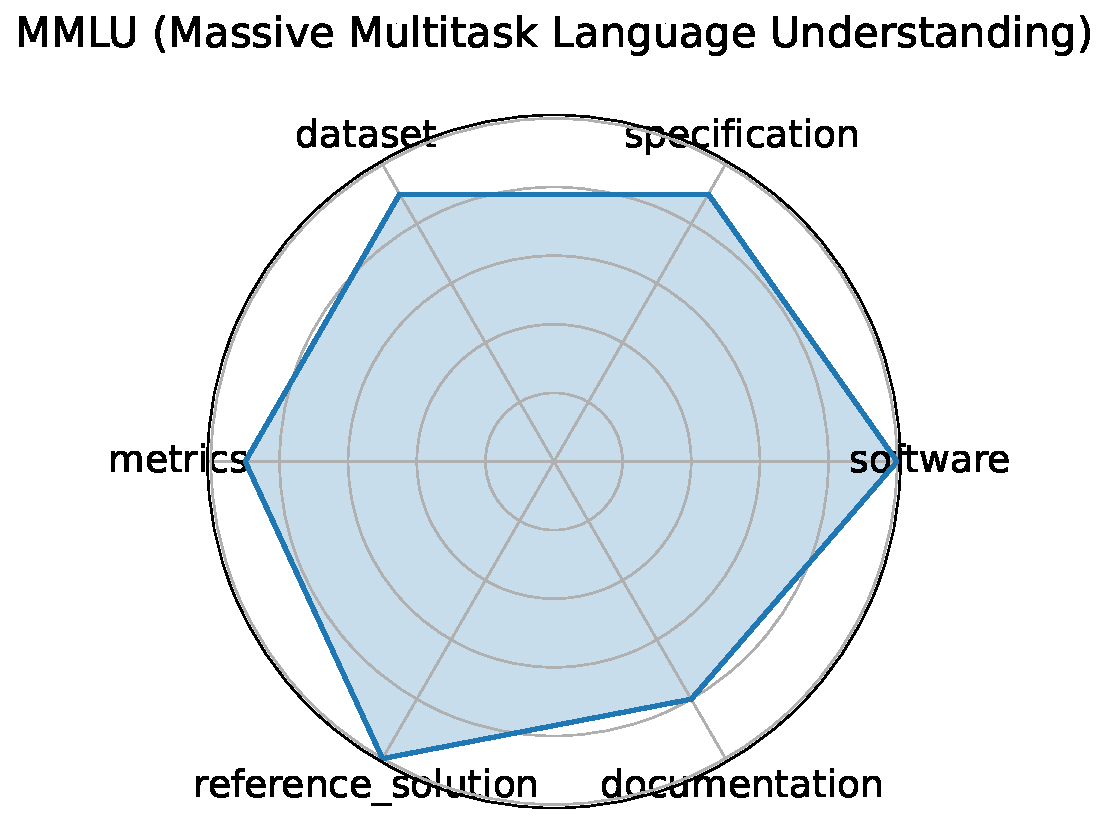
\includegraphics[width=0.15\textwidth]{mmlu_massive_multitask_language_understanding_radar.pdf} & MMLU (Massive Multitask Language Understanding) & Multidomain & Academic knowledge and reasoning across 57 subjects & multitask, multiple-choice, zero-shot, few-shot, knowledge probing & Multiple choice & General reasoning, subject-matter understanding & Accuracy & GPT-4o, Gemini 1.5 Pro, o1, DeepSeek-R1 & \cite{hendrycks2021measuring}\href{https://paperswithcode.com/dataset/mmlu}{$\Rightarrow$} \\ \hline
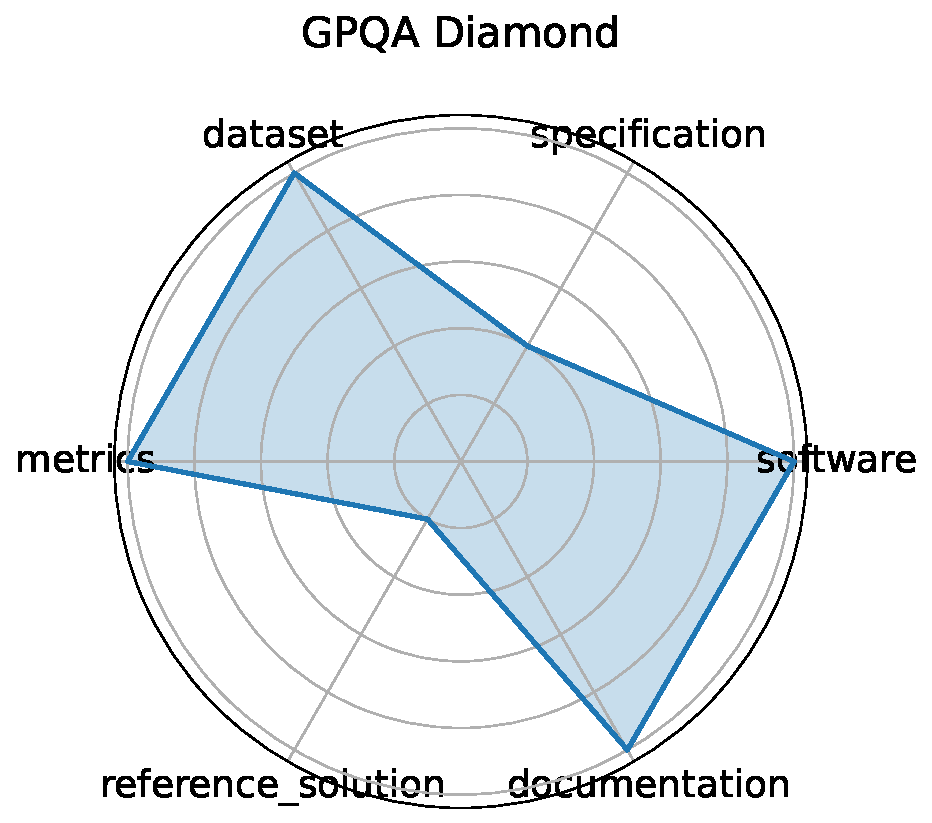
\includegraphics[width=0.15\textwidth]{gpqa_diamond_radar.pdf} & GPQA Diamond & Science & Graduate-level scientific reasoning & Google-proof, graduate-level, science QA, chemistry, physics & Multiple choice, Multi-step QA & Scientific reasoning, deep knowledge & Accuracy & o1, DeepSeek-R1 & \cite{rein2023gpqagraduatelevelgoogleproofqa}\href{https://arxiv.org/abs/2311.12022}{$\Rightarrow$} \\ \hline
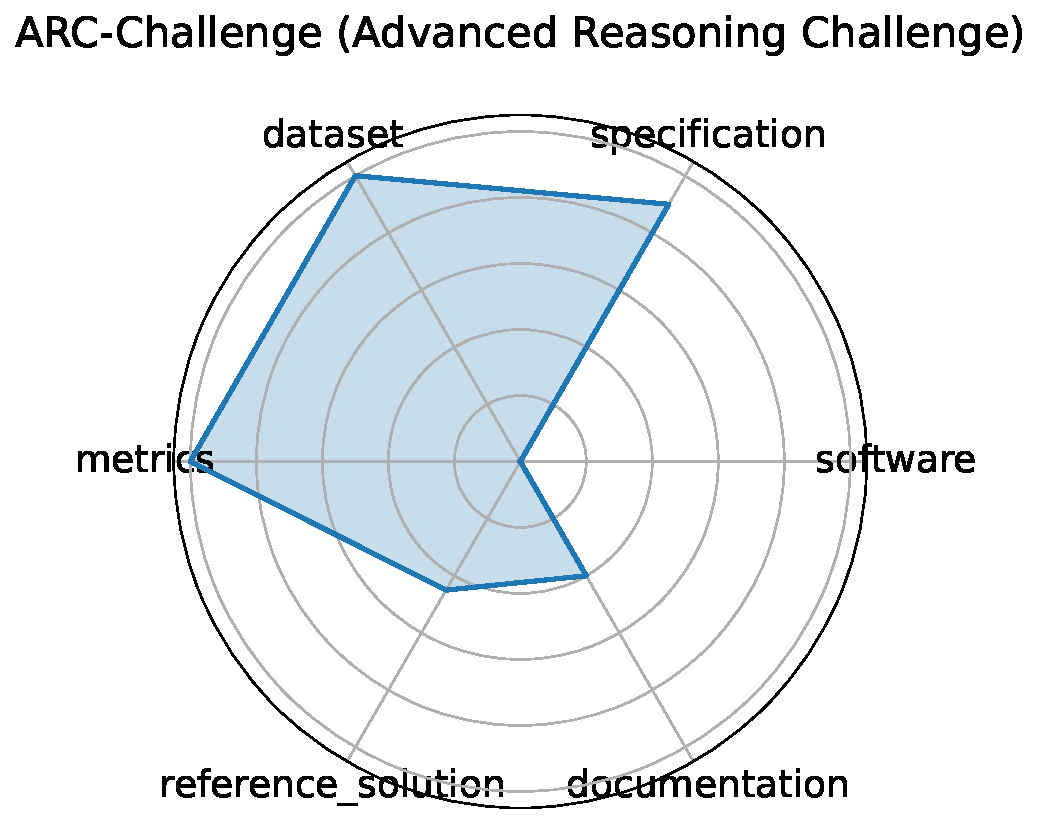
\includegraphics[width=0.15\textwidth]{arc-challenge_advanced_reasoning_challenge_radar.pdf} & ARC-Challenge (Advanced Reasoning Challenge) & Science & Grade-school science with reasoning emphasis & grade-school, science QA, challenge set, reasoning & Multiple choice & Commonsense and scientific reasoning & Accuracy & GPT-4, Claude & \cite{clark2018think}\href{https://allenai.org/data/arc}{$\Rightarrow$} \\ \hline
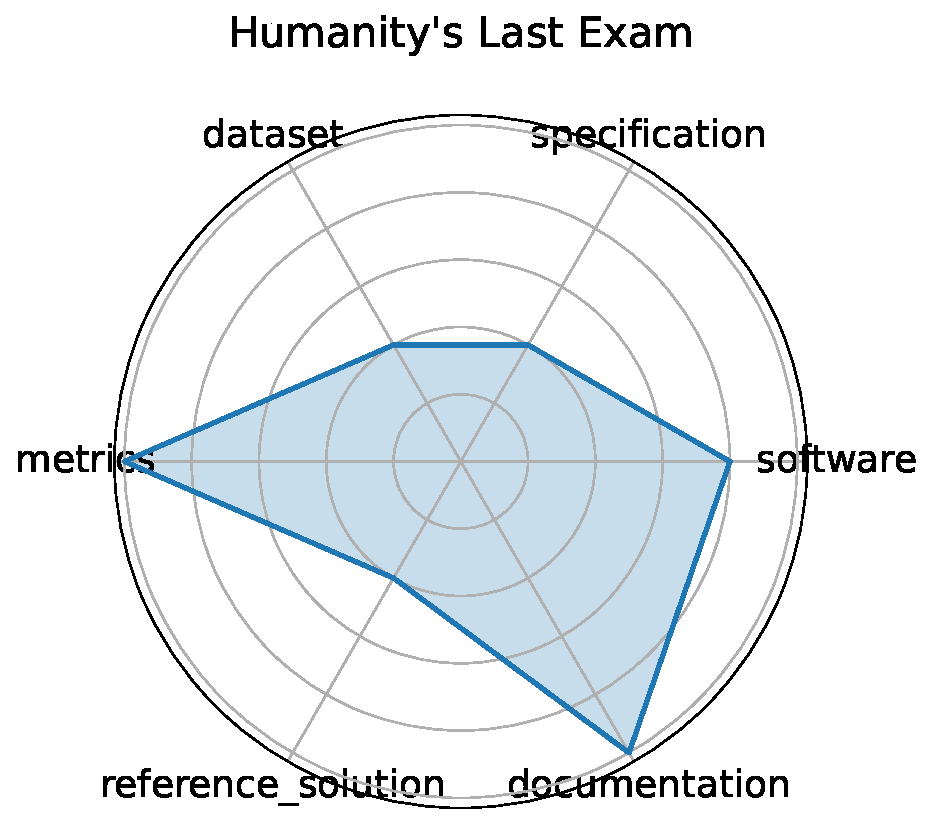
\includegraphics[width=0.15\textwidth]{humanitys_last_exam_radar.pdf} & Humanity's Last Exam & Multidomain & Broad cross-domain academic reasoning & cross-domain, academic exam, multiple-choice, multidisciplinary & Multiple choice & Cross-domain academic reasoning & Accuracy & \cite{phan2025humanitysexam}\href{https://arxiv.org/abs/2501.14249}{$\Rightarrow$} \\ \hline
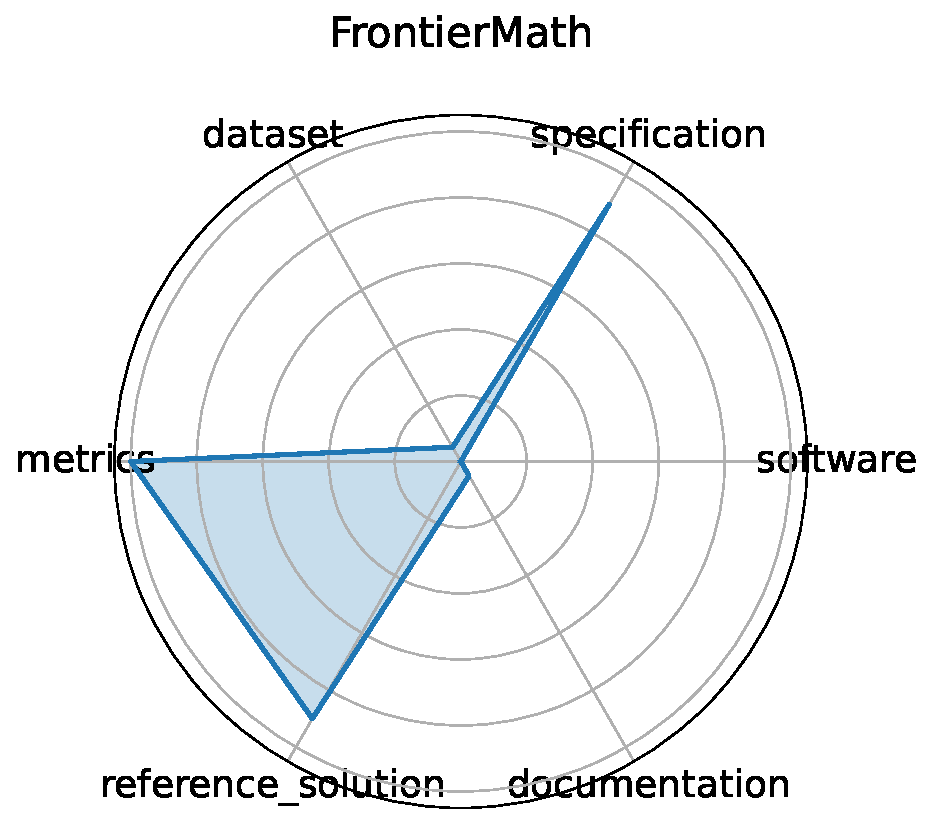
\includegraphics[width=0.15\textwidth]{frontiermath_radar.pdf} & FrontierMath & Mathematics & Challenging advanced mathematical reasoning & symbolic reasoning, number theory, algebraic geometry, category theory & Problem solving & Symbolic and abstract mathematical reasoning & Accuracy & \cite{glazer2024frontiermathbenchmarkevaluatingadvanced}\href{https://arxiv.org/abs/2411.04872}{$\Rightarrow$} \\ \hline
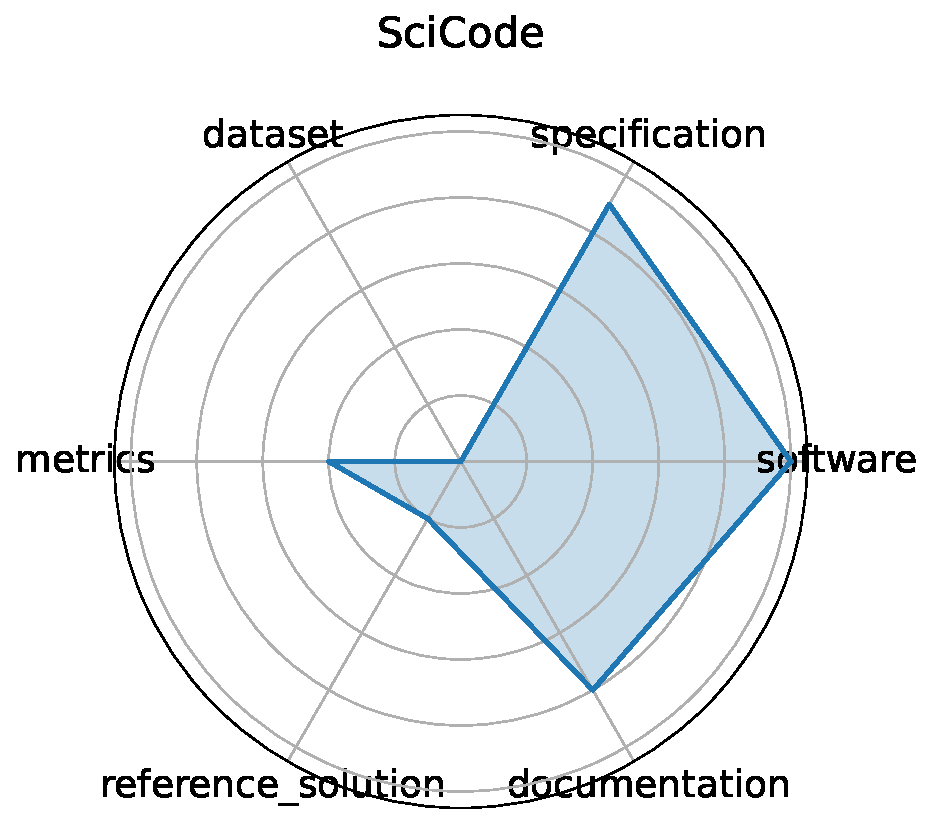
\includegraphics[width=0.15\textwidth]{scicode_radar.pdf} & SciCode & Scientific Programming & Scientific code generation and problem solving & code synthesis, scientific computing, programming benchmark & Coding & Program synthesis, scientific computing & Solve rate (\%) & Claude3.5-Sonnet & \cite{tian2024scicoderesearchcodingbenchmark}\href{https://arxiv.org/abs/2407.13168}{$\Rightarrow$} \\ \hline
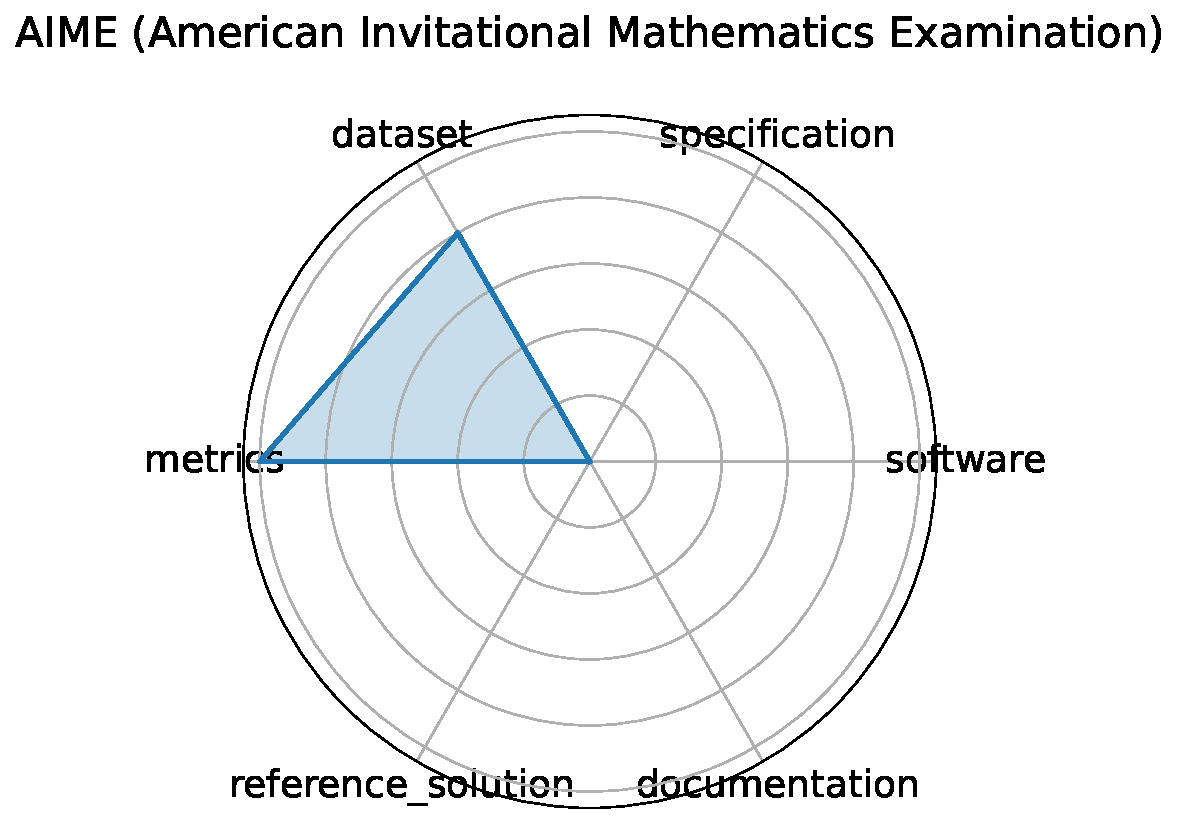
\includegraphics[width=0.15\textwidth]{aime_american_invitational_mathematics_examination_radar.pdf} & AIME (American Invitational Mathematics Examination) & Mathematics & Pre-college advanced problem solving & algebra, combinatorics, number theory, geometry & Problem solving & Mathematical problem-solving and reasoning & Accuracy & \cite{www-aime}\href{https://artofproblemsolving.com/wiki/index.php/AIME\_Problems\_and\_Solutions}{$\Rightarrow$} \\ \hline
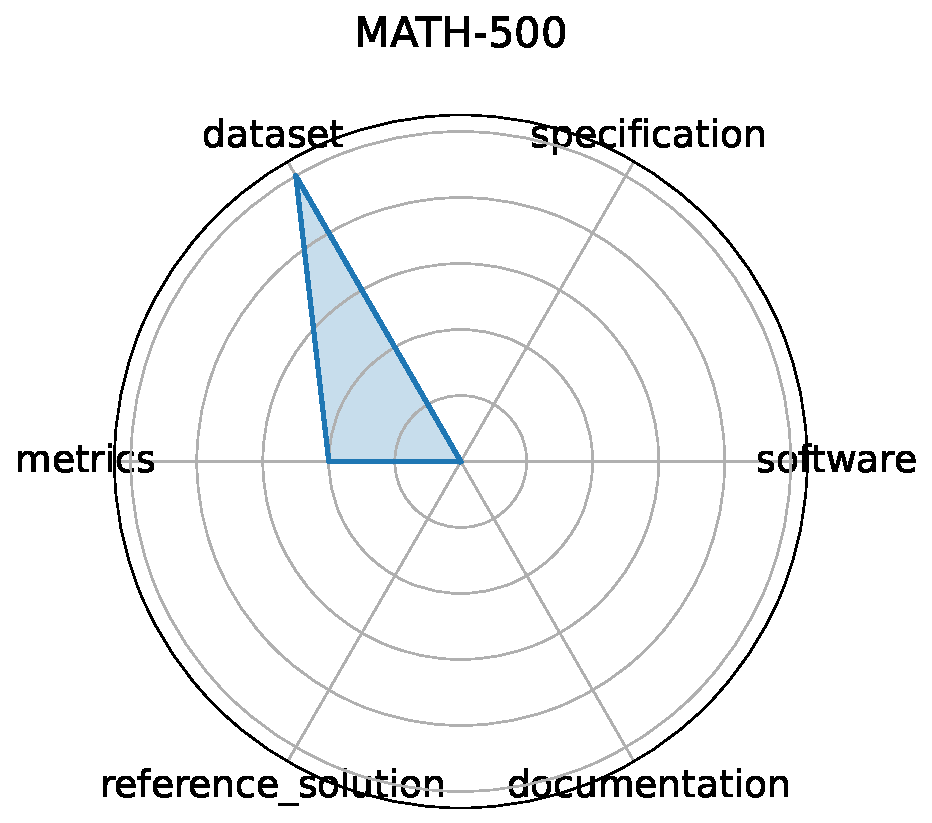
\includegraphics[width=0.15\textwidth]{math-_radar.pdf} & MATH-500 & Mathematics & Math reasoning generalization & calculus, algebra, number theory, geometry & Problem solving & Math reasoning and generalization & Accuracy & \cite{huggingface2025math500}\href{https://huggingface.co/datasets/HuggingFaceH4/MATH-500}{$\Rightarrow$} \\ \hline
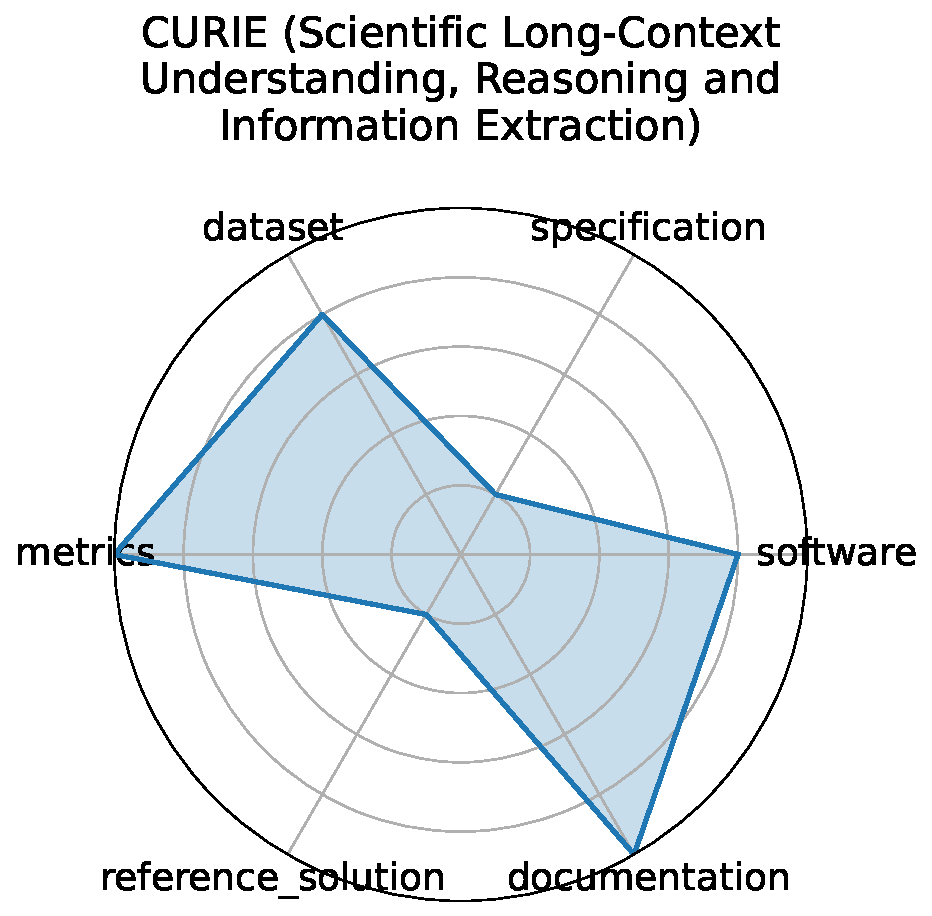
\includegraphics[width=0.15\textwidth]{curie_scientific_long-context_understanding_reasoning_and_information_extraction_radar.pdf} & CURIE (Scientific Long-Context Understanding, Reasoning and Information Extraction) & Multidomain Science & Long-context scientific reasoning & long-context, information extraction, multimodal & Information extraction, Reasoning, Concept tracking, Aggregation, Algebraic manipulation, Multimodal comprehension & Long-context understanding and scientific reasoning & Accuracy & \cite{curie2024}\href{https://arxiv.org/abs/2404.02029}{$\Rightarrow$} \\ \hline
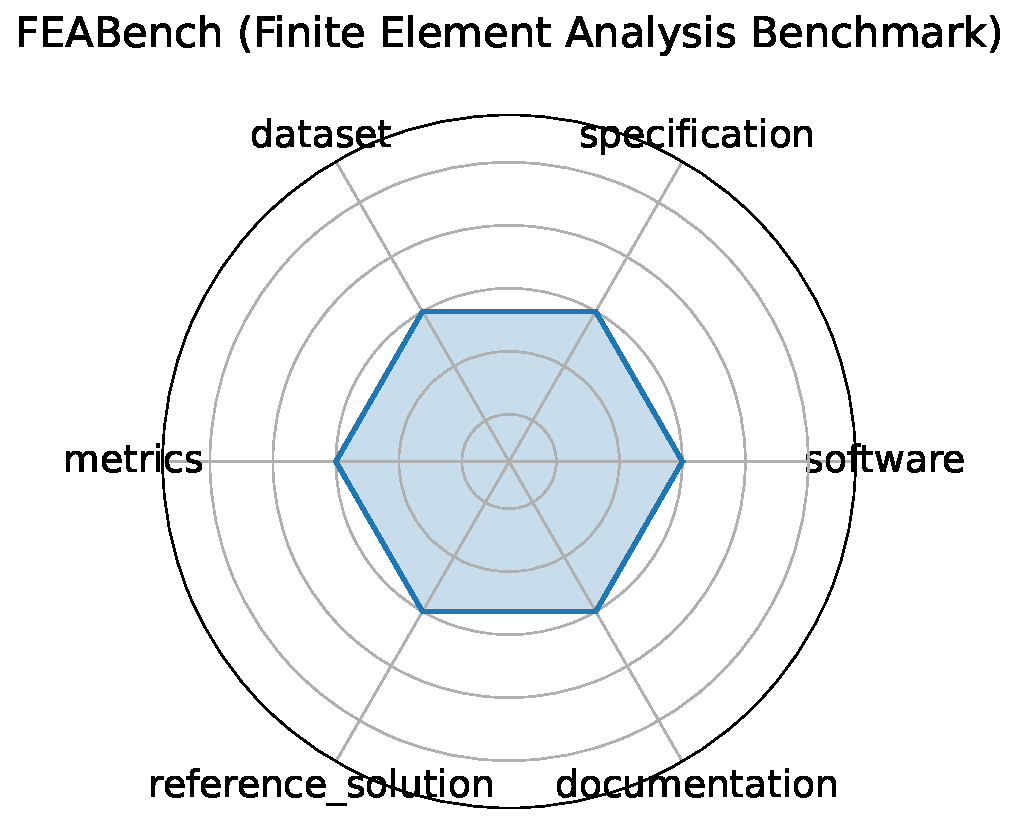
\includegraphics[width=0.15\textwidth]{feabench_finite_element_analysis_benchmark_radar.pdf} & FEABench (Finite Element Analysis Benchmark) & Computational Engineering & FEA simulation accuracy and performance & finite element, simulation, PDE & Simulation, Performance evaluation & Numerical simulation accuracy and efficiency & Solve time, Error norm & FEniCS, deal.II & \cite{allen2023feabench}\href{https://github.com/alleninstitute/feabench}{$\Rightarrow$} \\ \hline
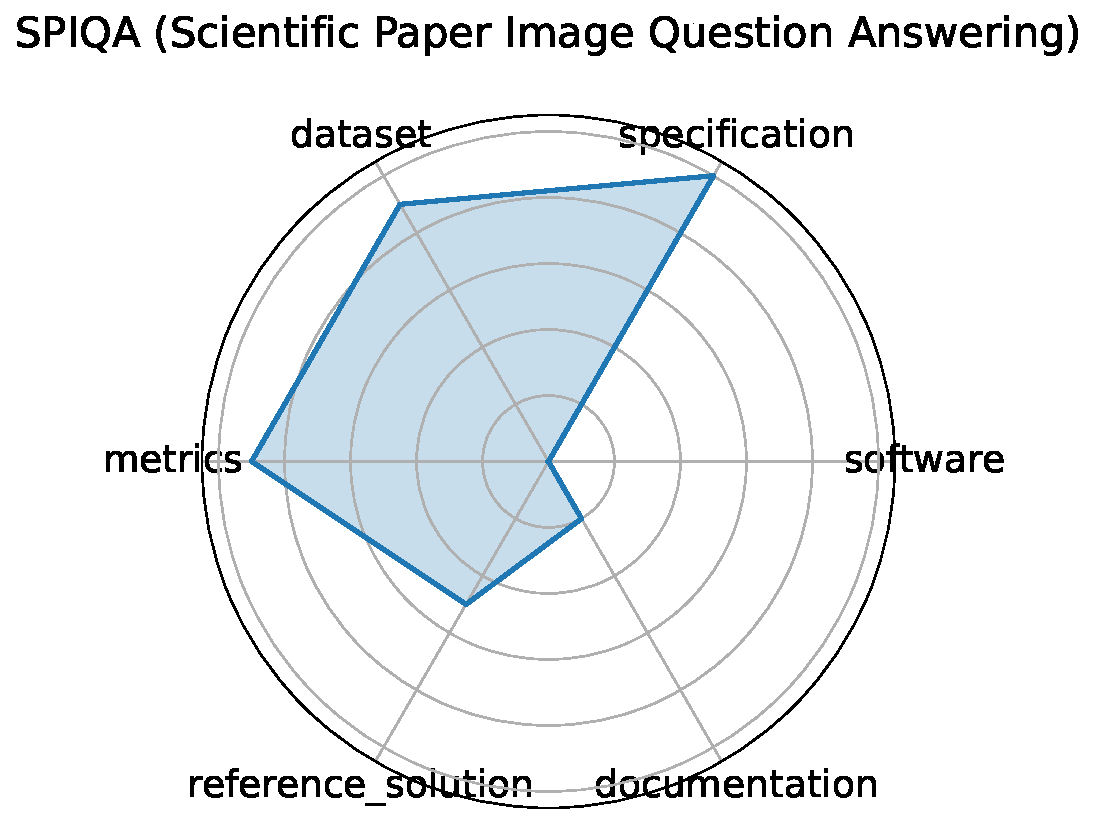
\includegraphics[width=0.15\textwidth]{spiqa_scientific_paper_image_question_answering_radar.pdf} & SPIQA (Scientific Paper Image Question Answering) & Computer Science & Multimodal QA on scientific figures & multimodal QA, figure understanding, table comprehension, chain-of-thought & Question answering, Multimodal QA, Chain-of-Thought evaluation & Visual-textual reasoning in scientific contexts & Accuracy, F1 score & Chain-of-Thought models, Multimodal QA systems & \cite{zhong2024spiqa}\href{https://arxiv.org/abs/2407.09413}{$\Rightarrow$} \\ \hline
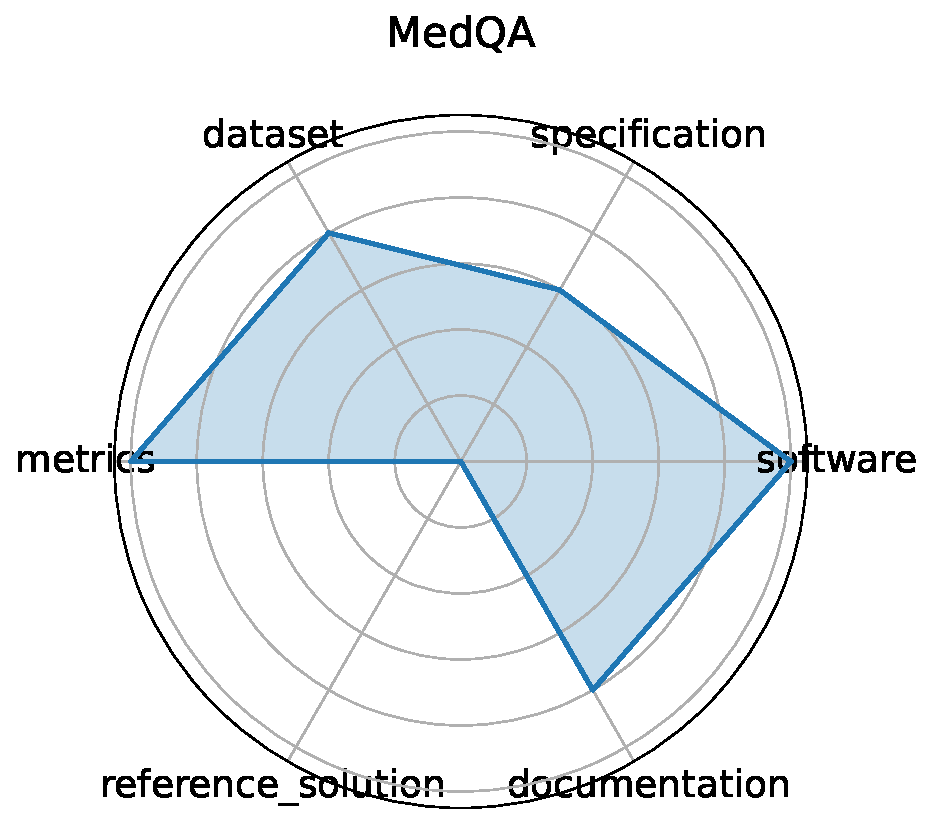
\includegraphics[width=0.15\textwidth]{medqa_radar.pdf} & MedQA & Medical Question Answering & Medical board exam QA & USMLE, diagnostic QA, medical knowledge, multilingual & Multiple choice & Medical diagnosis and knowledge retrieval & Accuracy & Neural reader, Retrieval-based QA systems & \cite{jin2020diseasedoespatienthave}\href{https://arxiv.org/abs/2009.13081}{$\Rightarrow$} \\ \hline
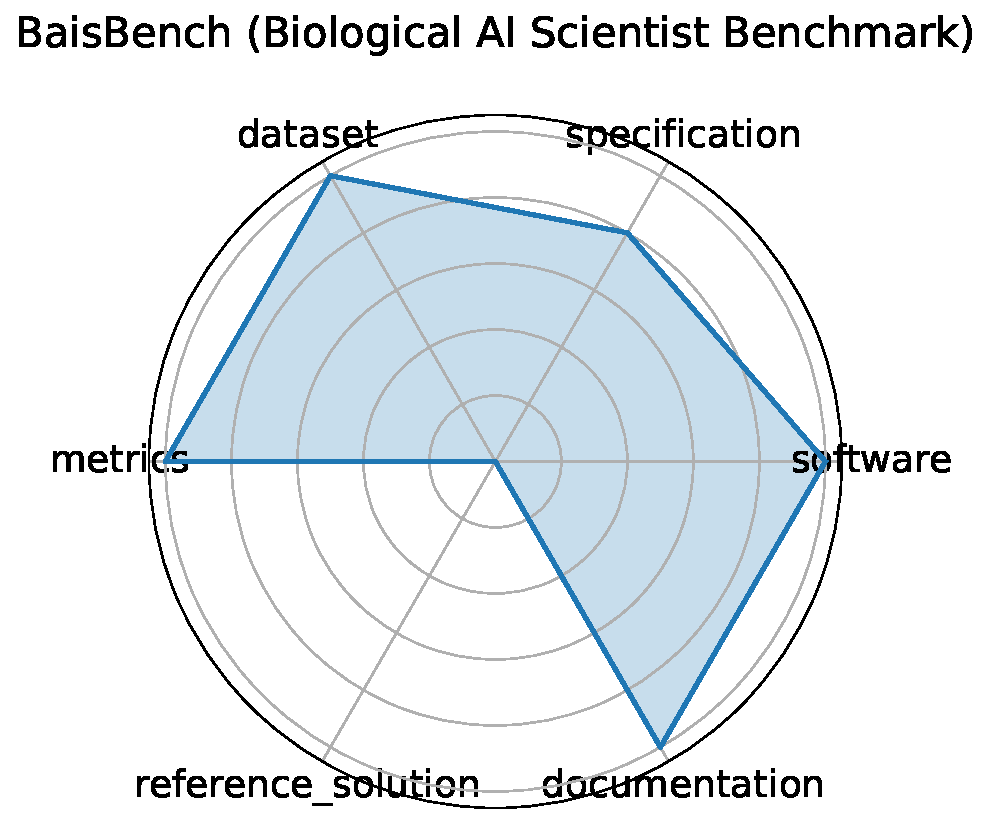
\includegraphics[width=0.15\textwidth]{baisbench_biological_ai_scientist_benchmark_radar.pdf} & BaisBench (Biological AI Scientist Benchmark) & Computational Biology & Omics-driven AI research tasks & single-cell annotation, biological QA, autonomous discovery & Cell type annotation, Multiple choice & Autonomous biological research capabilities & Annotation accuracy, QA accuracy & LLM-based AI scientist agents & \cite{luo2025benchmarkingaiscientistsomics}\href{https://arxiv.org/abs/2505.08341}{$\Rightarrow$} \\ \hline
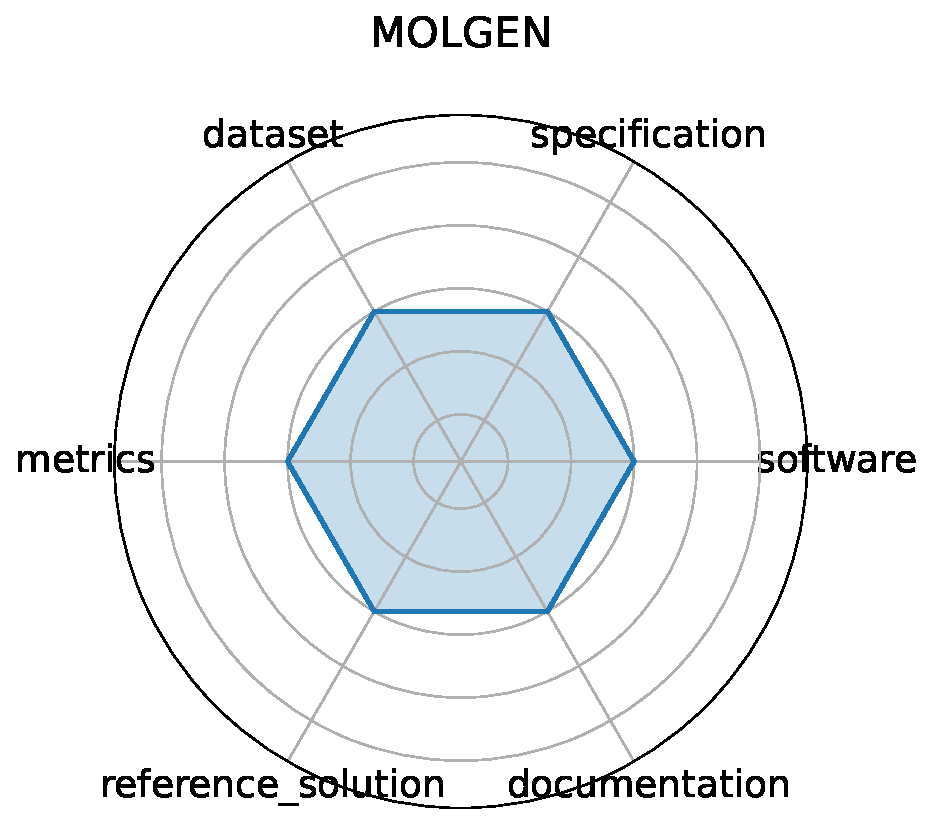
\includegraphics[width=0.15\textwidth]{molgen_radar.pdf} & MOLGEN & Computational Chemistry & Molecular generation and optimization & SELFIES, GAN, property optimization & Distribution learning, Goal-oriented generation & Generation of valid and optimized molecular structures & Validity\%, Novelty\%, QED, Docking score & MolGen & \cite{fang2024domainagnosticmoleculargenerationchemical}\href{https://github.com/zjunlp/MolGen}{$\Rightarrow$} \\ \hline
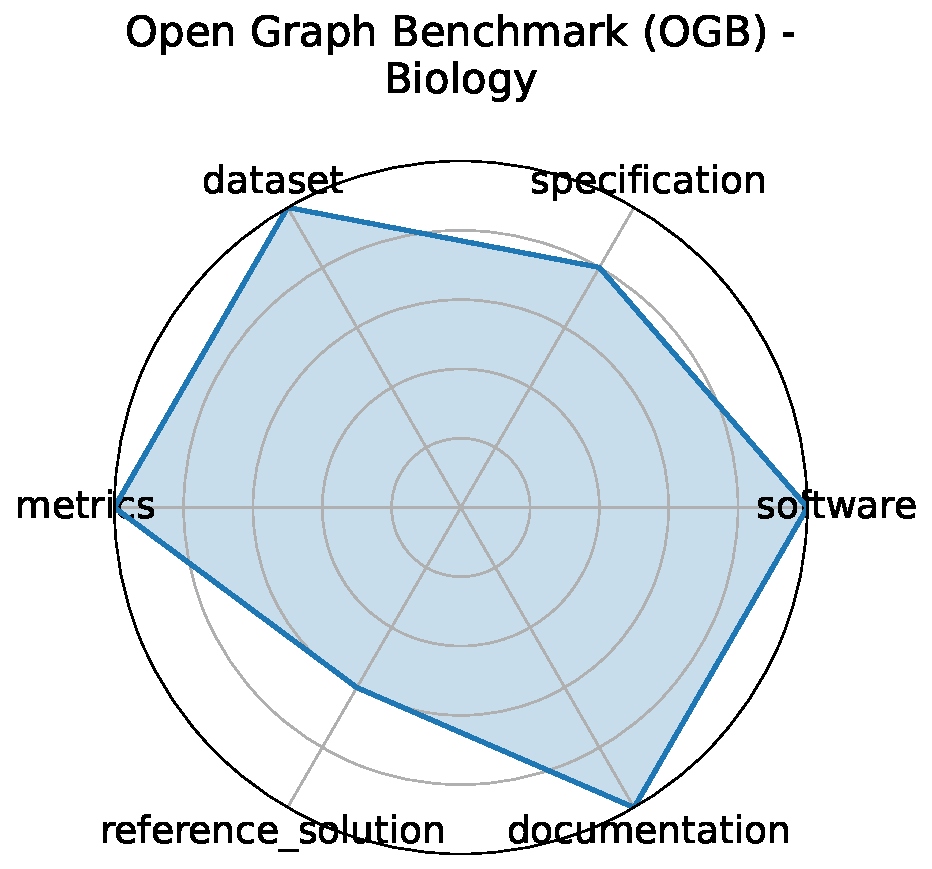
\includegraphics[width=0.15\textwidth]{open_graph_benchmark_ogb_-_biology_radar.pdf} & Open Graph Benchmark (OGB) - Biology & Graph ML & Biological graph property prediction & node prediction, link prediction, graph classification & Node property prediction, Link property prediction, Graph property prediction & Scalability and generalization in graph ML for biology & Accuracy, ROC-AUC & GCN, GraphSAGE, GAT & \cite{hu2021opengraphbenchmarkdatasets}\href{https://ogb.stanford.edu/docs/home/}{$\Rightarrow$} \\ \hline
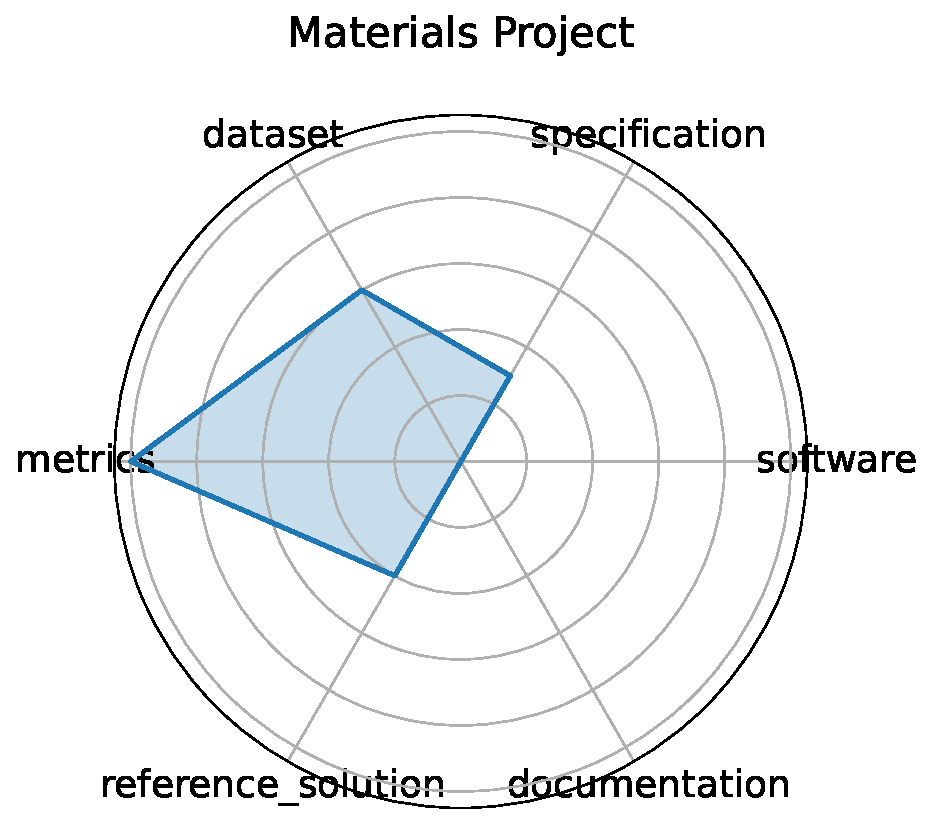
\includegraphics[width=0.15\textwidth]{materials_project_radar.pdf} & Materials Project & Materials Science & DFT-based property prediction & DFT, materials genome, high-throughput & Property prediction & Prediction of inorganic material properties & MAE, R{\texttwosuperior} & Automatminer, Crystal Graph Neural Networks & \cite{jain2013materials}\href{https://materialsproject.org/}{$\Rightarrow$} \\ \hline
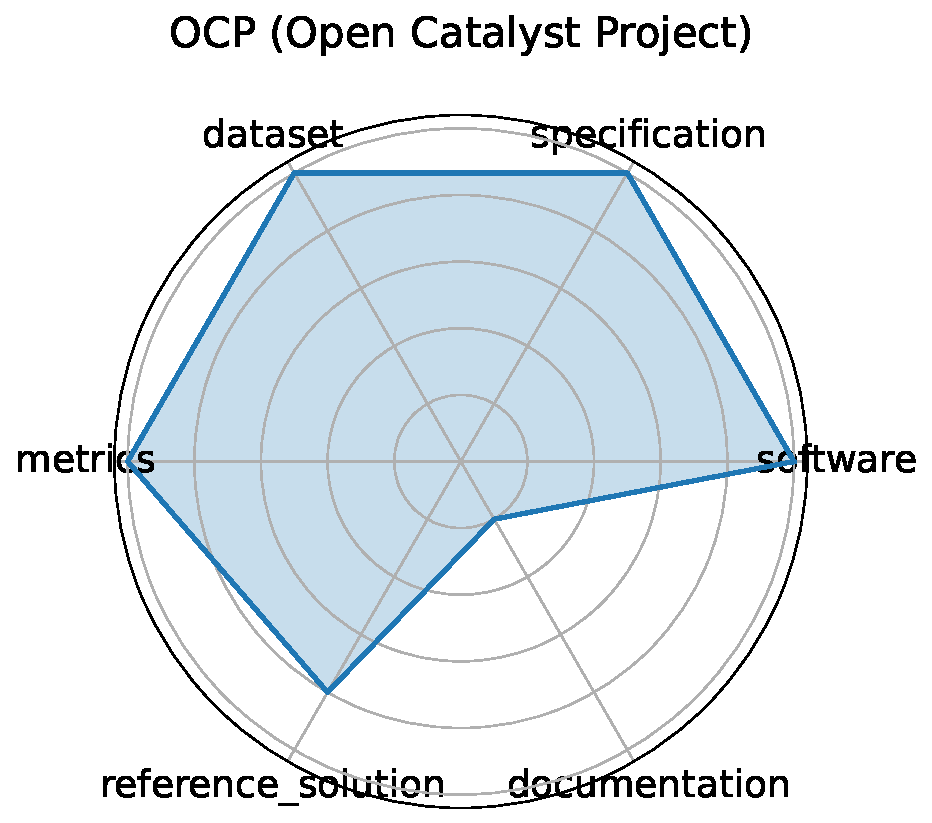
\includegraphics[width=0.15\textwidth]{ocp_open_catalyst_project_radar.pdf} & OCP (Open Catalyst Project) & Chemistry; Materials Science & Catalyst adsorption energy prediction & DFT relaxations, adsorption energy, graph neural networks & Energy prediction, Force prediction & Prediction of adsorption energies and forces & MAE (energy), MAE (force) & CGCNN, SchNet, DimeNet++, GemNet-OC & \cite{chanussot2021oc20,tran2023oc22,doi:10.1021/acscatal.0c04525,tran2023b}\href{https://opencatalystproject.org/}{$\Rightarrow$} \\ \hline
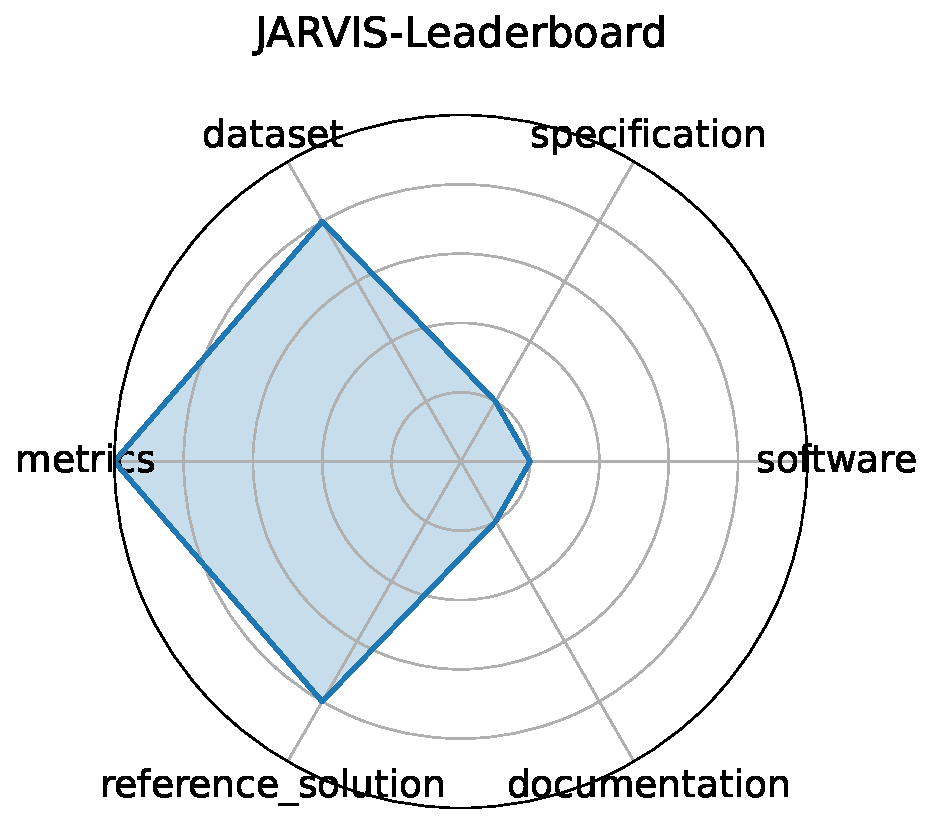
\includegraphics[width=0.15\textwidth]{jarvis-leaderboard_radar.pdf} & JARVIS-Leaderboard & Materials Science; Benchmarking & Comparative evaluation of materials design methods & leaderboards, materials methods, simulation & Method benchmarking, Leaderboard ranking & Performance comparison across diverse materials design methods & MAE, RMSE, Accuracy & \cite{choudhary2024jarvis}\href{https://arxiv.org/abs/2306.11688}{$\Rightarrow$} \\ \hline
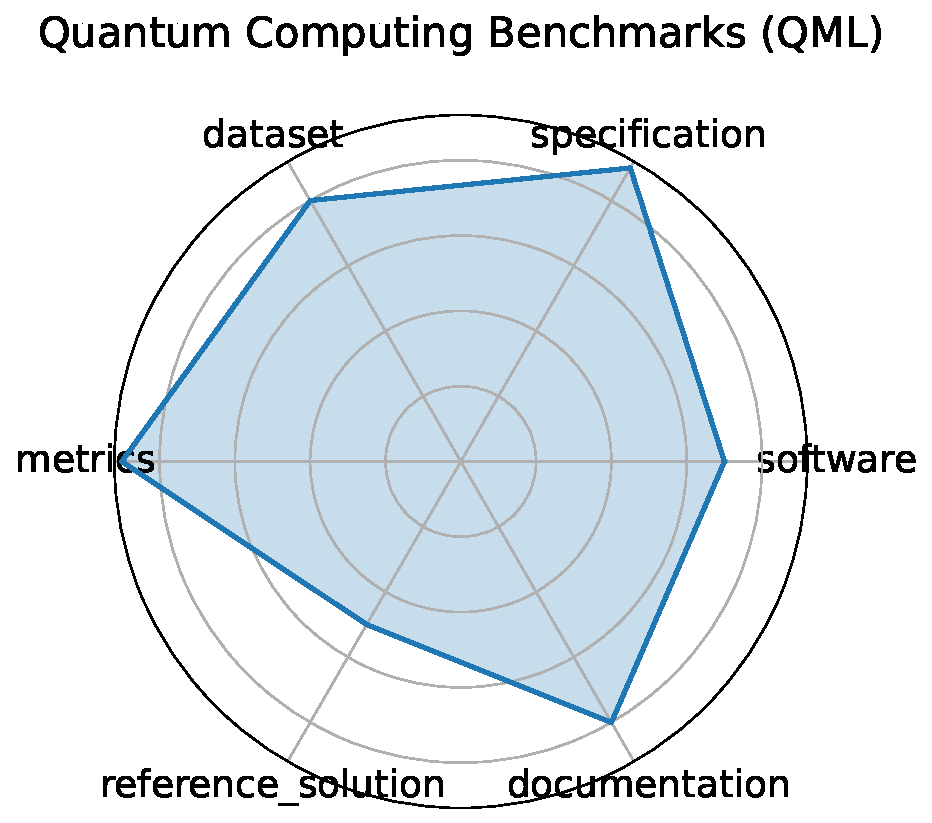
\includegraphics[width=0.15\textwidth]{quantum_computing_benchmarks_qml_radar.pdf} & Quantum Computing Benchmarks (QML) & Quantum Computing & Quantum algorithm performance evaluation & quantum circuits, state preparation, error correction & Circuit benchmarking, State classification & Quantum algorithm performance and fidelity & Fidelity, Success probability & IBM Q, IonQ, AQT@LBNL & \cite{kiwit2023}\href{['https://github.com/XanaduAI/qml-benchmarks', 'https://pennylane.ai/datasets/collection/qml-benchmarks']}{$\Rightarrow$} \\ \hline
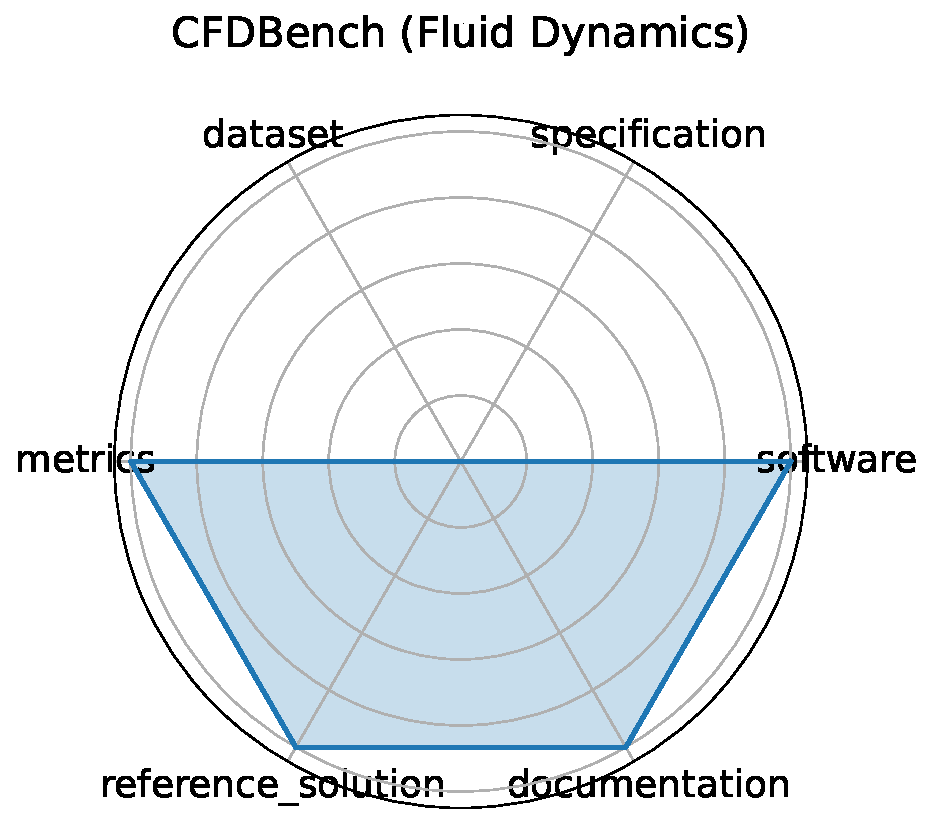
\includegraphics[width=0.15\textwidth]{cfdbench_fluid_dynamics_radar.pdf} & CFDBench (Fluid Dynamics) & Fluid Dynamics; Scientific ML & Neural operator surrogate modeling & neural operators, CFD, FNO, DeepONet & Surrogate modeling & Generalization of neural operators for PDEs & L2 error, MAE & FNO, DeepONet, U-Net & \cite{luo2024cfdbenchlargescalebenchmarkmachine}\href{https://arxiv.org/abs/2310.05963}{$\Rightarrow$} \\ \hline
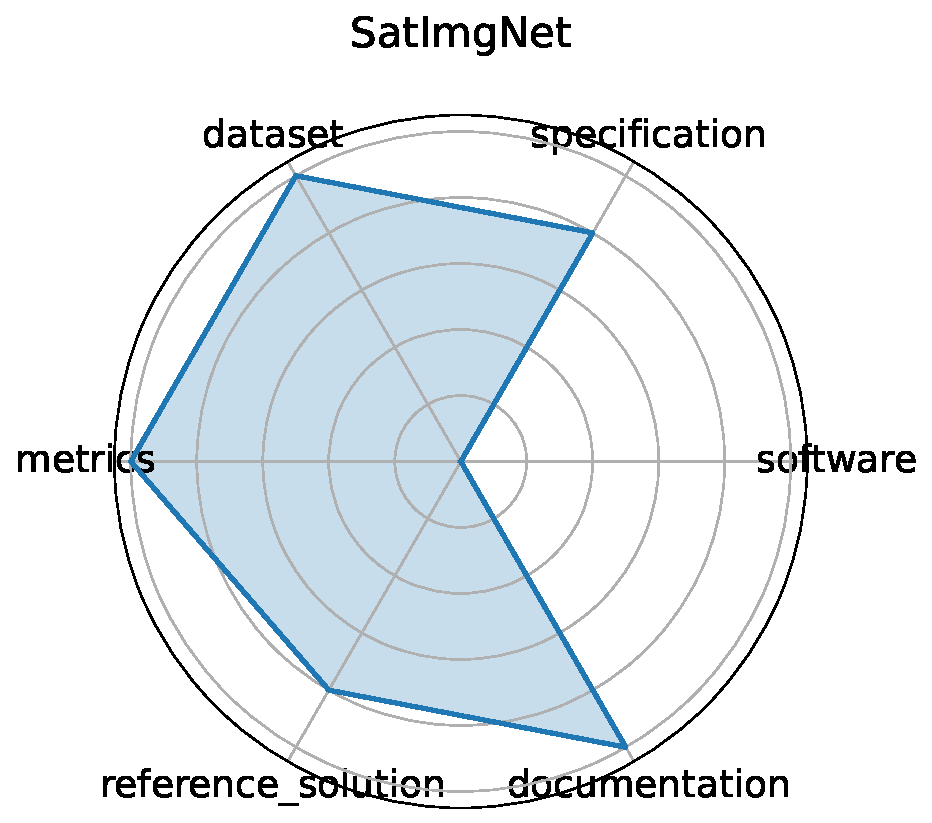
\includegraphics[width=0.15\textwidth]{satimgnet_radar.pdf} & SatImgNet & Remote Sensing & Satellite imagery classification & land-use, zero-shot, multi-task & Image classification & Zero-shot land-use classification & Accuracy & \cite{roberts2023satinmultitaskmetadatasetclassifying} \\ \hline
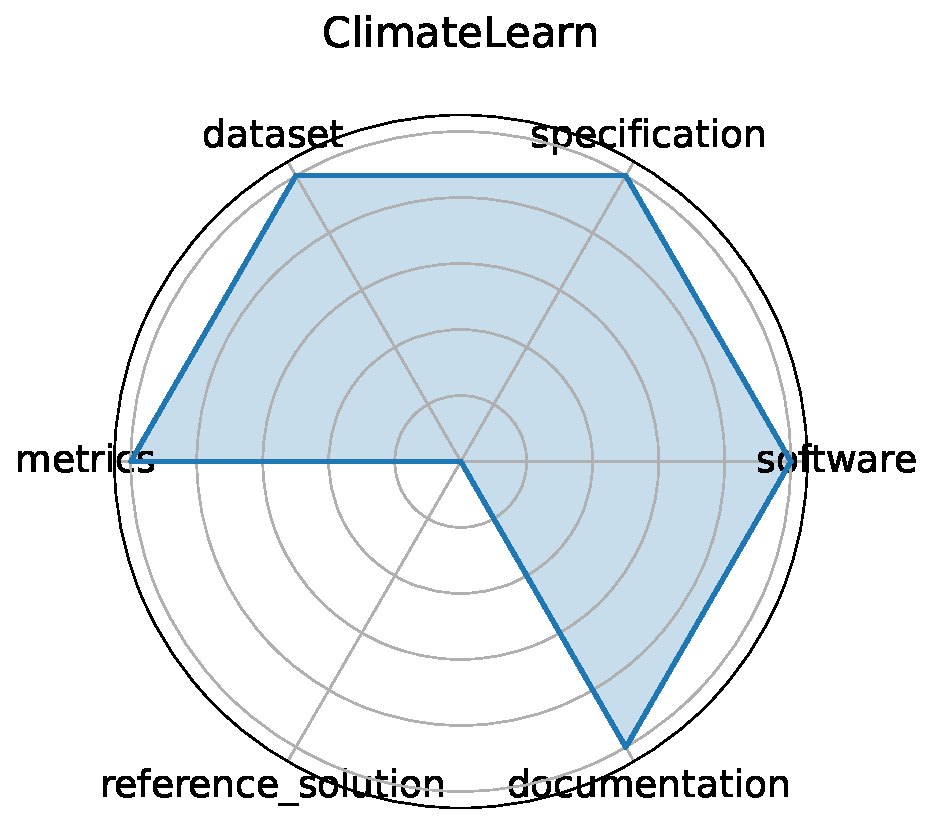
\includegraphics[width=0.15\textwidth]{climatelearn_radar.pdf} & ClimateLearn & Climate Science; Forecasting & ML for weather and climate modeling & medium-range forecasting, ERA5, data-driven & Forecasting & Global weather prediction (3-5 days) & RMSE, Anomaly correlation & CNN baselines, ResNet variants & \cite{nguyen2023climatelearnbenchmarkingmachinelearning}\href{https://arxiv.org/abs/2307.01909}{$\Rightarrow$} \\ \hline
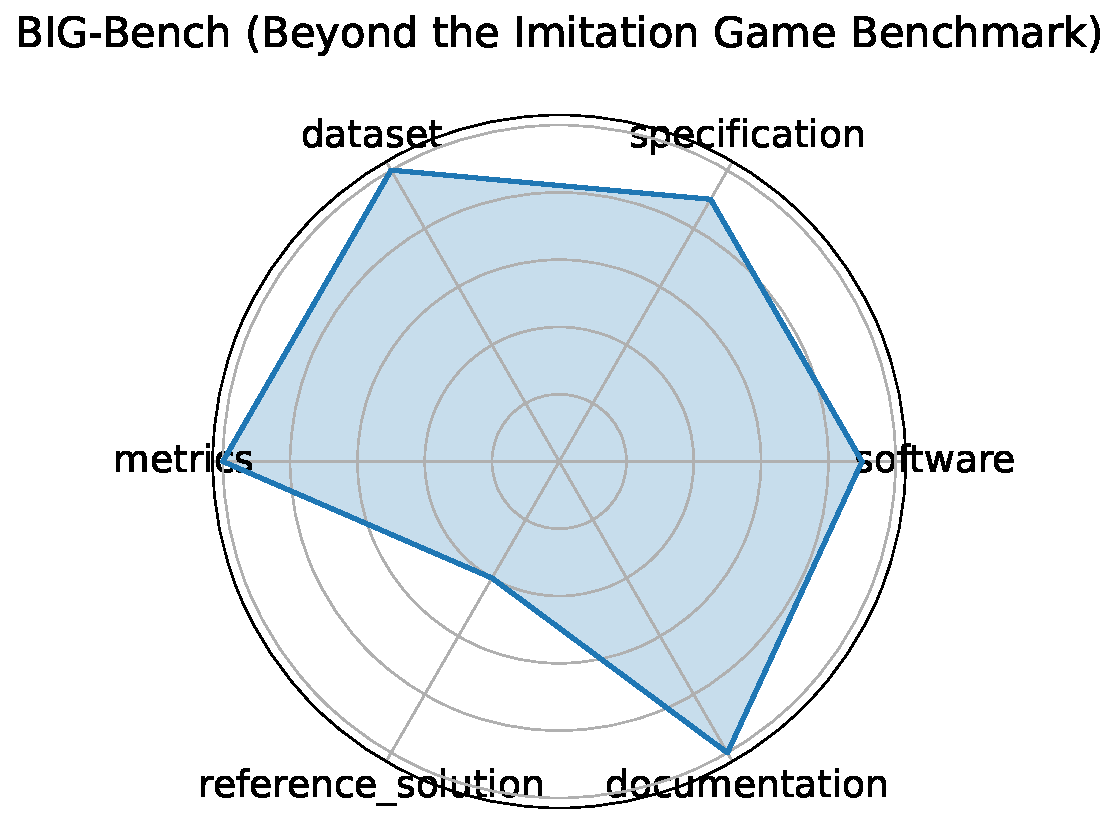
\includegraphics[width=0.15\textwidth]{big-bench_beyond_the_imitation_game_benchmark_radar.pdf} & BIG-Bench (Beyond the Imitation Game Benchmark) & NLP; AI Evaluation & Diverse reasoning and generalization tasks & few-shot, multi-task, bias analysis & Few-shot evaluation, Multi-task evaluation & Reasoning and generalization across diverse tasks & Accuracy, Task-specific metrics & GPT-3, Dense Transformers, Sparse Transformers & \cite{srivastava2023imitationgamequantifyingextrapolating}\href{https://github.com/google/BIG-bench}{$\Rightarrow$} \\ \hline
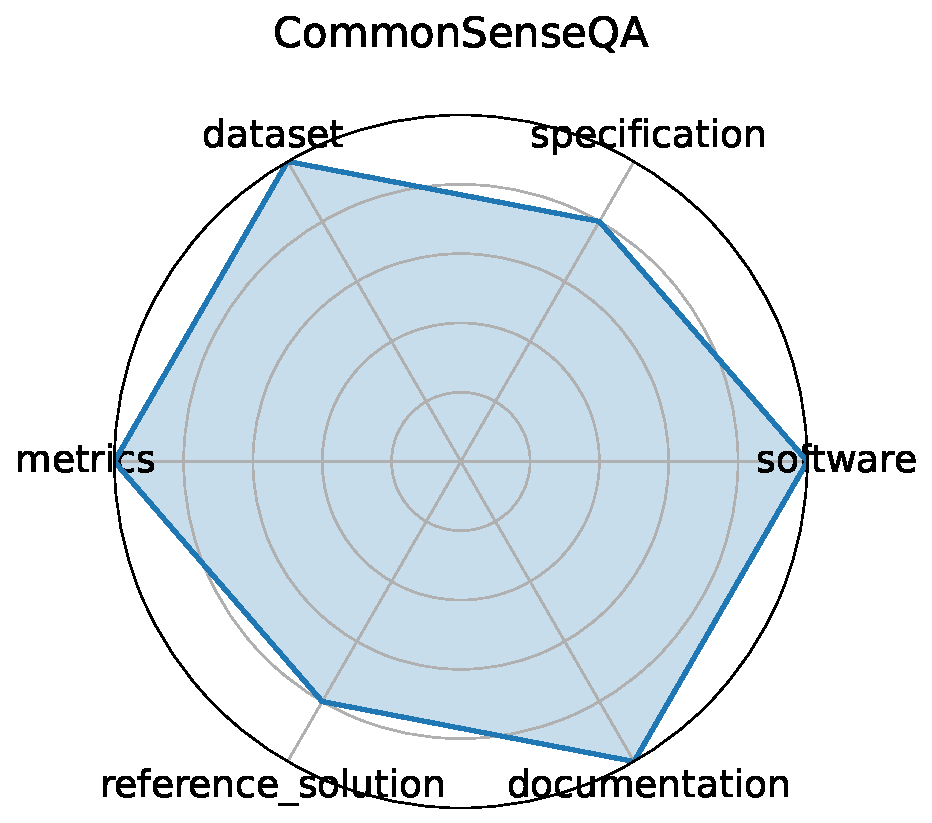
\includegraphics[width=0.15\textwidth]{commonsenseqa_radar.pdf} & CommonSenseQA & NLP; Commonsense & Commonsense question answering & ConceptNet, multiple-choice, adversarial & Multiple choice & Commonsense reasoning and knowledge integration & Accuracy & BERT-large, RoBERTa, GPT-3 & \cite{talmor2019commonsenseqaquestionansweringchallenge}\href{https://paperswithcode.com/paper/commonsenseqa-a-question-answering-challenge}{$\Rightarrow$} \\ \hline
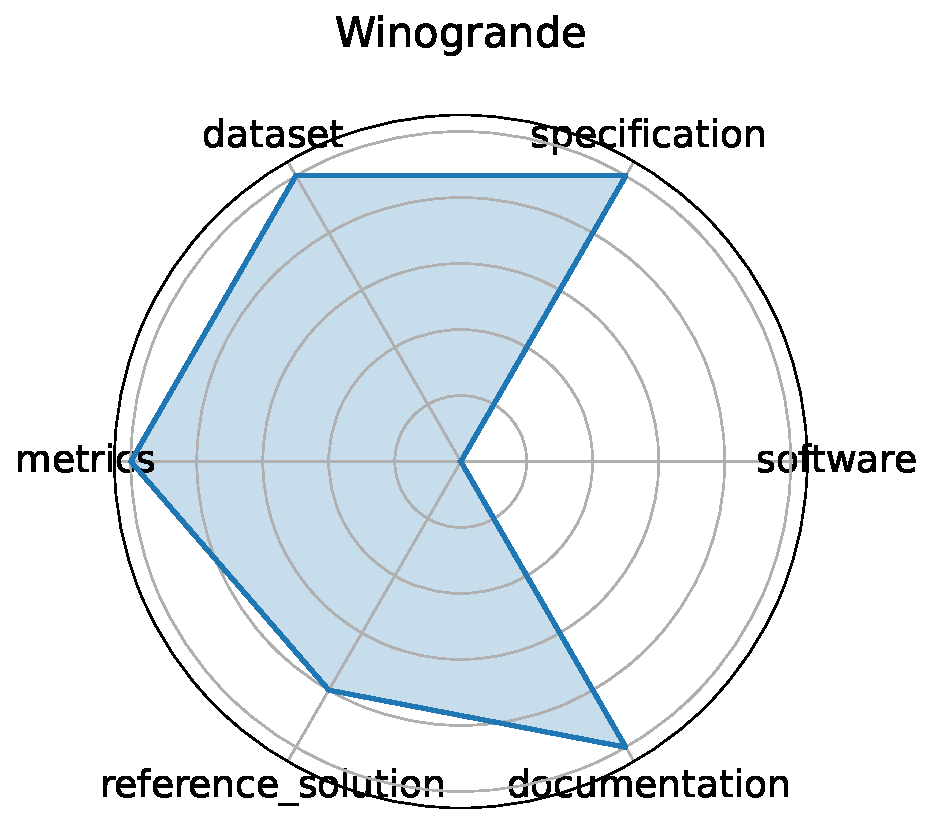
\includegraphics[width=0.15\textwidth]{winogrande_radar.pdf} & Winogrande & NLP; Commonsense & Winograd Schema-style pronoun resolution & adversarial, pronoun resolution & Pronoun resolution & Robust commonsense reasoning & Accuracy, AUC & RoBERTa, BERT, GPT-2 & \cite{sakaguchi2019winograndeadversarialwinogradschema}\href{https://leaderboard.allenai.org/winogrande/submissions/public}{$\Rightarrow$} \\ \hline
\end{longtable}
}

\end{landscape}
